\section{Mechanical Design}
\subsection*{Problem Definition}
\begin{frame}
\frametitle{Problem Definition}
\begin{block}{Features}
\begin{itemize}
\item
SLOM concept, 2D / 3D hopping\\[0.2in]
\item
Tension springs instead of compression spring\\[0.2in]
\item
Reduce leg mass, higher hopping heights\\[0.2in]
\item
Reaction wheel\\[0.1in]
\begin{itemize}
    \item
    Necessary for inplace hopping\\[0.1in]
    \item
    Stable running gait\\[0.1in]
\end{itemize}
\item
Onboard embedded system
\end{itemize}
\end{block}
\end{frame}

\subsection*{Design 1}
\begin{frame}
\frametitle{Design 1}
\begin{columns}

\column{0.5\textwidth}
\begin{figure}
\centering
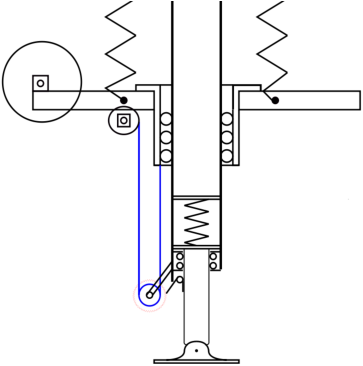
\includegraphics[width=\textwidth]{fig/pratik_des.pdf}
\caption{Winch pulley design}
\end{figure}

\column{0.5\textwidth}
\begin{block}{Features}
\begin{itemize}
\item
{\greencol EPM :}\\[0.1in]
    \begin{itemize}
    \item
    Motor pulls itself down\\[0.1in]
    \item
    Moves twice the extension\\[0.1in]
    \end{itemize}
\item
{\greencol Constraint :}\\[0.1in]
    \begin{itemize}
    \item
    Toothed pulley constrained by the hatch\\[0.1in]
    \item
    Impact pushes hatch inside\\[0.1in]
    \item
    Momentum transfer\\[0.1in]
    \end{itemize}
\end{itemize}
\end{block}

\end{columns}
\end{frame}

\begin{frame}
\frametitle{Design 1}
\begin{columns}
\column{0.5\textwidth}
\begin{figure}
\centering
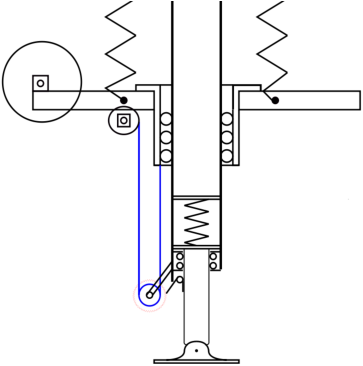
\includegraphics[width=\textwidth]{fig/pratik_des.pdf}
\caption{Winch pulley design}
\end{figure}

\column{0.5\textwidth}
\begin{block}{Evaluation}
\begin{itemize}
\item
{\greencol Pros :}\\[0.1in]
    \begin{itemize}
    \item
    Simple constraint mechanism\\[0.1in]
    \item
    Easier to make a light leg\\[0.1in]
    \end{itemize}
\item
\alert{Cons} :\\[0.1in]
    \begin{itemize}
    \item
    Winch can slide off the pulley\\[0.1in]
    \item
    Torsion spring : potentional point of failure\\[0.1in]
    \item
    Torques on roller bearings\\[0.1in]
    \end{itemize}
\end{itemize}
\end{block}
\end{columns}
\end{frame}

\subsection*{Design 2}
\begin{frame}
\frametitle{Design 2}
\begin{columns}

\column{0.5\textwidth}
\begin{figure}
\centering
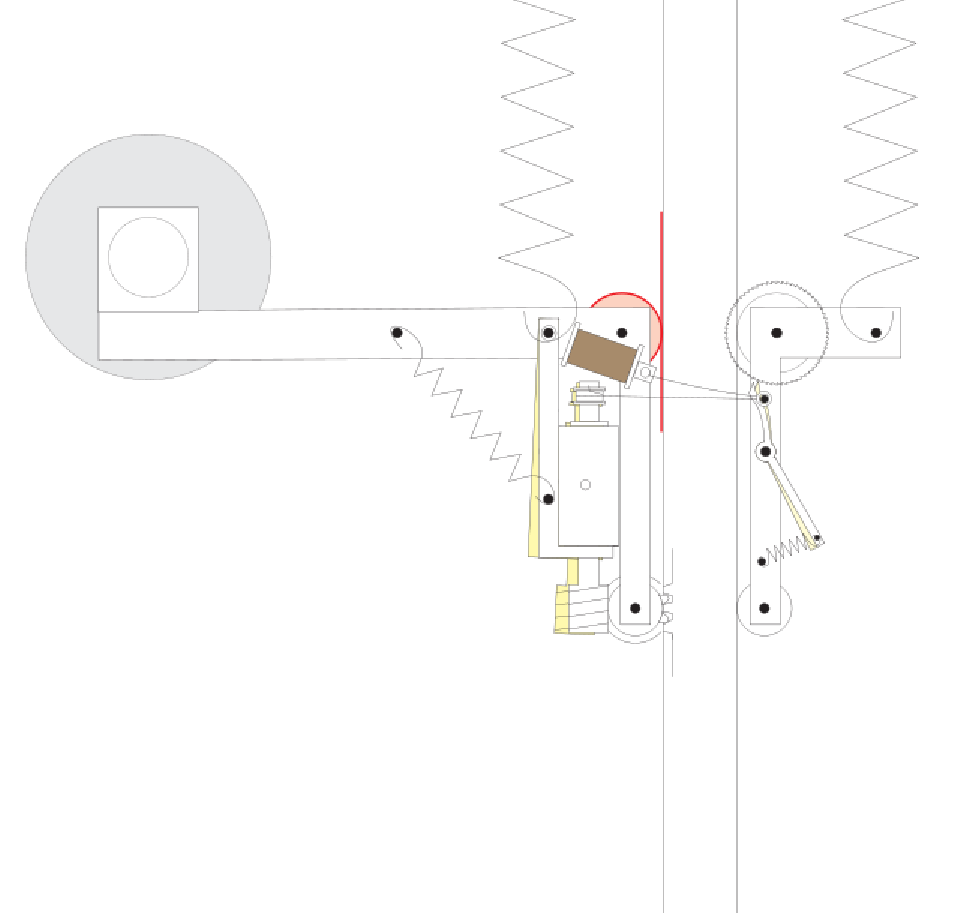
\includegraphics[width=\textwidth]{fig/seth_design.pdf}
\caption{Rack and pinion design}
\end{figure}

\column{0.5\textwidth}
\begin{block}{Features}
\begin{itemize}
\item
{\greencol EPM :}\\[0.1in]
    \begin{itemize}
    \item
    Rack worm-worm wheel\\[0.1in]
    \item
    Band drive\\[0.1in]
    \item
    Main spring can push the worm onto the rack\\[0.1in]
    \end{itemize}
\item
{\greencol Constraint :}\\[0.1in]
    \begin{itemize}
    \item
    Friction pulley\\[0.1in]
    \item
    Ratchet with paul\\[0.1in]
    \item
    Motor sleeve moves left\\[0.1in]
    \end{itemize}
\end{itemize}
\end{block}

\end{columns}
\end{frame}

\begin{frame}
\frametitle{Design 2}
\begin{columns}
\column{0.5\textwidth}
\begin{figure}
\centering
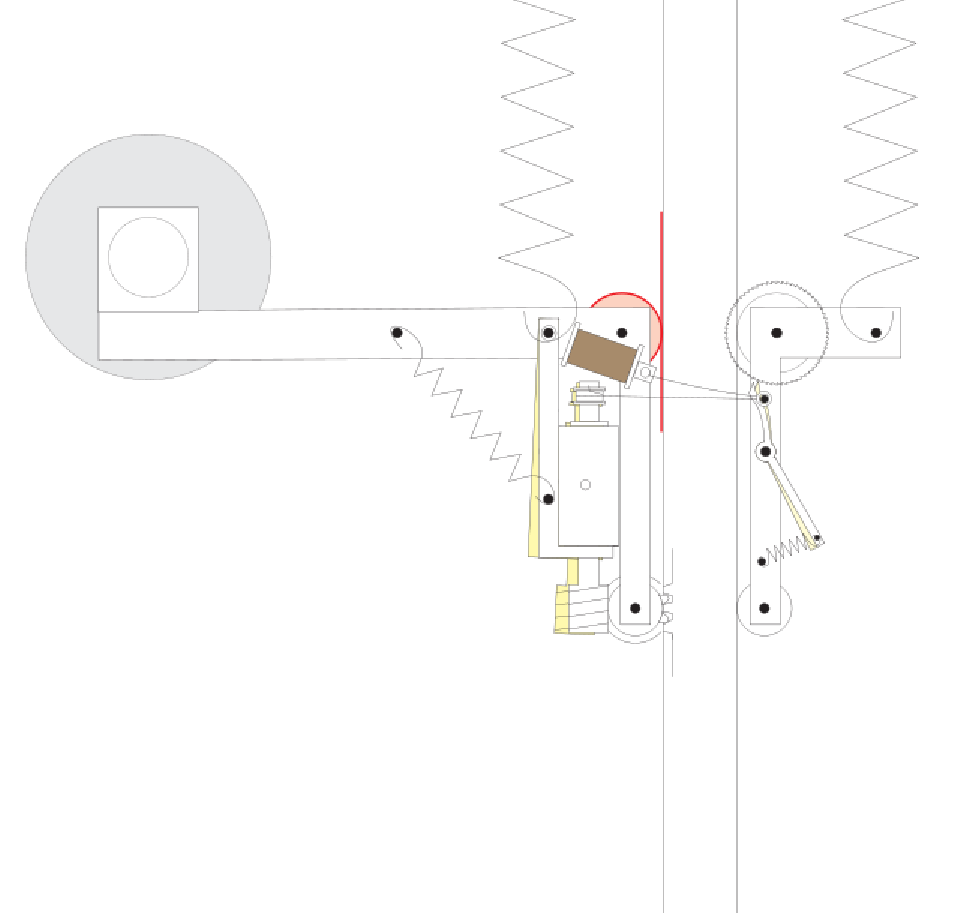
\includegraphics[width=\textwidth]{fig/seth_design.pdf}
\caption{Rack and pinion design}
\end{figure}

\column{0.5\textwidth}
\begin{block}{Evaluation}
\begin{itemize}
\item
{\greencol Pros :}\\[0.1in]
    \begin{itemize}
    \item
    Mechanical advantage\\[0.1in]
    \item
    Less moving parts, easier to build\\[0.1in]
    \end{itemize}
\item
\alert{Cons} :\\[0.1in]
    \begin{itemize}
    \item
    Friction pulley\\[0.1in]
    \item
    Lower resolution\\[0.1in]
    \end{itemize}
\end{itemize}
\end{block}
\end{columns}
\end{frame}

